\frame
{
\frametitle{}
\begin{center}
	\Huge{Introducción}
\end{center}
}

\frame
{
\frametitle{Introducción}
\Large{¿Qué \textbf{no} es Linux?}
\normalsize
\begin{center}
	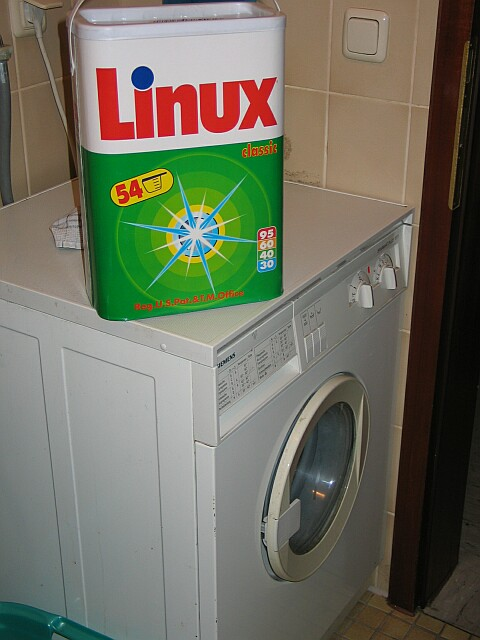
\includegraphics[width=4cm]{img/detergente-linux}
\end{center}
}

\frame
{
\frametitle{Introducción}
\Large{¿Qué \textbf{no} es Linux?}
\normalsize
15 Mitos sobre Linux
\begin{description}
	\item[1:] Si uso Linux me quedaré aislado del resto
	\item[2:] Linux no está estandarizado
	\item[3:] Sólo un experto programador puede instalar y usar Linux
	\item[4:] Linux está bien como juego, pero no para algo serio
	\item[5:] Linux no genera empleos
	\item[6:] Linux es feo
	\item[7:] En Linux no hay aplicaciones
	\item[8:] Linux es gratis y por tanto, lo que se haga en él no se puede cobrar
\end{description}
}
\frame
{
\frametitle{Introducción}
\Large{¿Qué \textbf{no} es Linux?}
\normalsize
15 Mitos sobre Linux
\begin{description}
	\item[9:] Linux es difícil de manejar
	\item[10:] En el software libre no hay innovación
	\item[11:] Todo mundo puede ver el código de los programas libres y por eso son inseguros
	\item[12:] El software libre es comunista
	\item[13:] No hay virus en Linux porque poca gente lo usa
	\item[14:] En linux no hay soporte
	\item[15:] Linux no le quita mercado a Windows, sino a Unix
\end{description}
}

\frame
{
\frametitle{Introducción}
\Large{¿Qué es Linux?}
\normalsize
\begin{itemize}
	\item Linux es un Sistema Operativo.
	\item No es el producto de una gran compañia.
	\item Es el resultado de una colaboracion entre compañias y personas.
	\item Se caracteriza por:
	\begin{itemize}
		\item Es gratis.
		\item Es libre.
		\item Es confiable.
		\item Es estable.
		\item Hay de todos los sabores.
	\end{itemize}
\end{itemize}
}
